\subsection{Composantes d'une cellule électrochimique}

\setcounter{equation}{0}
\setcounter{Q}{0}

\Q Donner une définition et expliciter le rôle joué par les composantes suivantes : électrode, demi-pile, solvant, électrolyte, séparateur et collecteur de courant.

Dans la suite de l'exercice, il s'agira d'identifier le rôle joué par chacune des composantes de différentes technologies de piles.

\solution{
\textbf{Electrode} : Une électrode est un conducteur électronique captant ou délivrant des électrons. \\
%\textbf{Cahier des charges :}
%\begin{itemize}
%\item Bon conducteur électronique ;
%\item Bon conducteur ionique si mécanisme d'insertion ;
%\item 
%\end{itemize} 
\textbf{Demi-pile} : Sous-compartiment de la cellule contenant une électrode et une solution. \\
\textbf{Solvant} : Espèce électroinactive pouvant solubiliser les espèces rédox et les espèces électrolytiques. \\
\textbf{Electrolyte} : Espèce électroinactive permettant la conduction ionique (aussi appelée migration) au sein de la cellule.
Il peut arriver parfois que l'électrolyte, comme dans la technologie Li-ion, soit une ou des espèces du système rédox. \\
\textbf{Collecteur de courant} : Matériau faisant la jonction électrique entre la partie électrique et l'électrode.
}

\Q La pile Daniell, développée en 1836 par John Daniell, est une cellule contenant un électrolyte acide en milieu aqueux et deux électrodes en zinc et en cuivre. Il s'agit d'une pile en solution aqueuse, qui peut être réalisée à l'aide d'un bécher où est placée un vase poreux en céramique. 

\begin{center}
\begin{minipage}{0.48\textwidth}

\includegraphics[width=\textwidth]{Ex35/Fig01}
\end{minipage}\hfill\begin{minipage}{0.48\textwidth}
\captionof{figure}{Schéma d'une pile Daniell}
\end{minipage}
\end{center}

\solution{On peut proposer la légende suivante : 
\begin{center}
\begin{minipage}{0.48\textwidth}
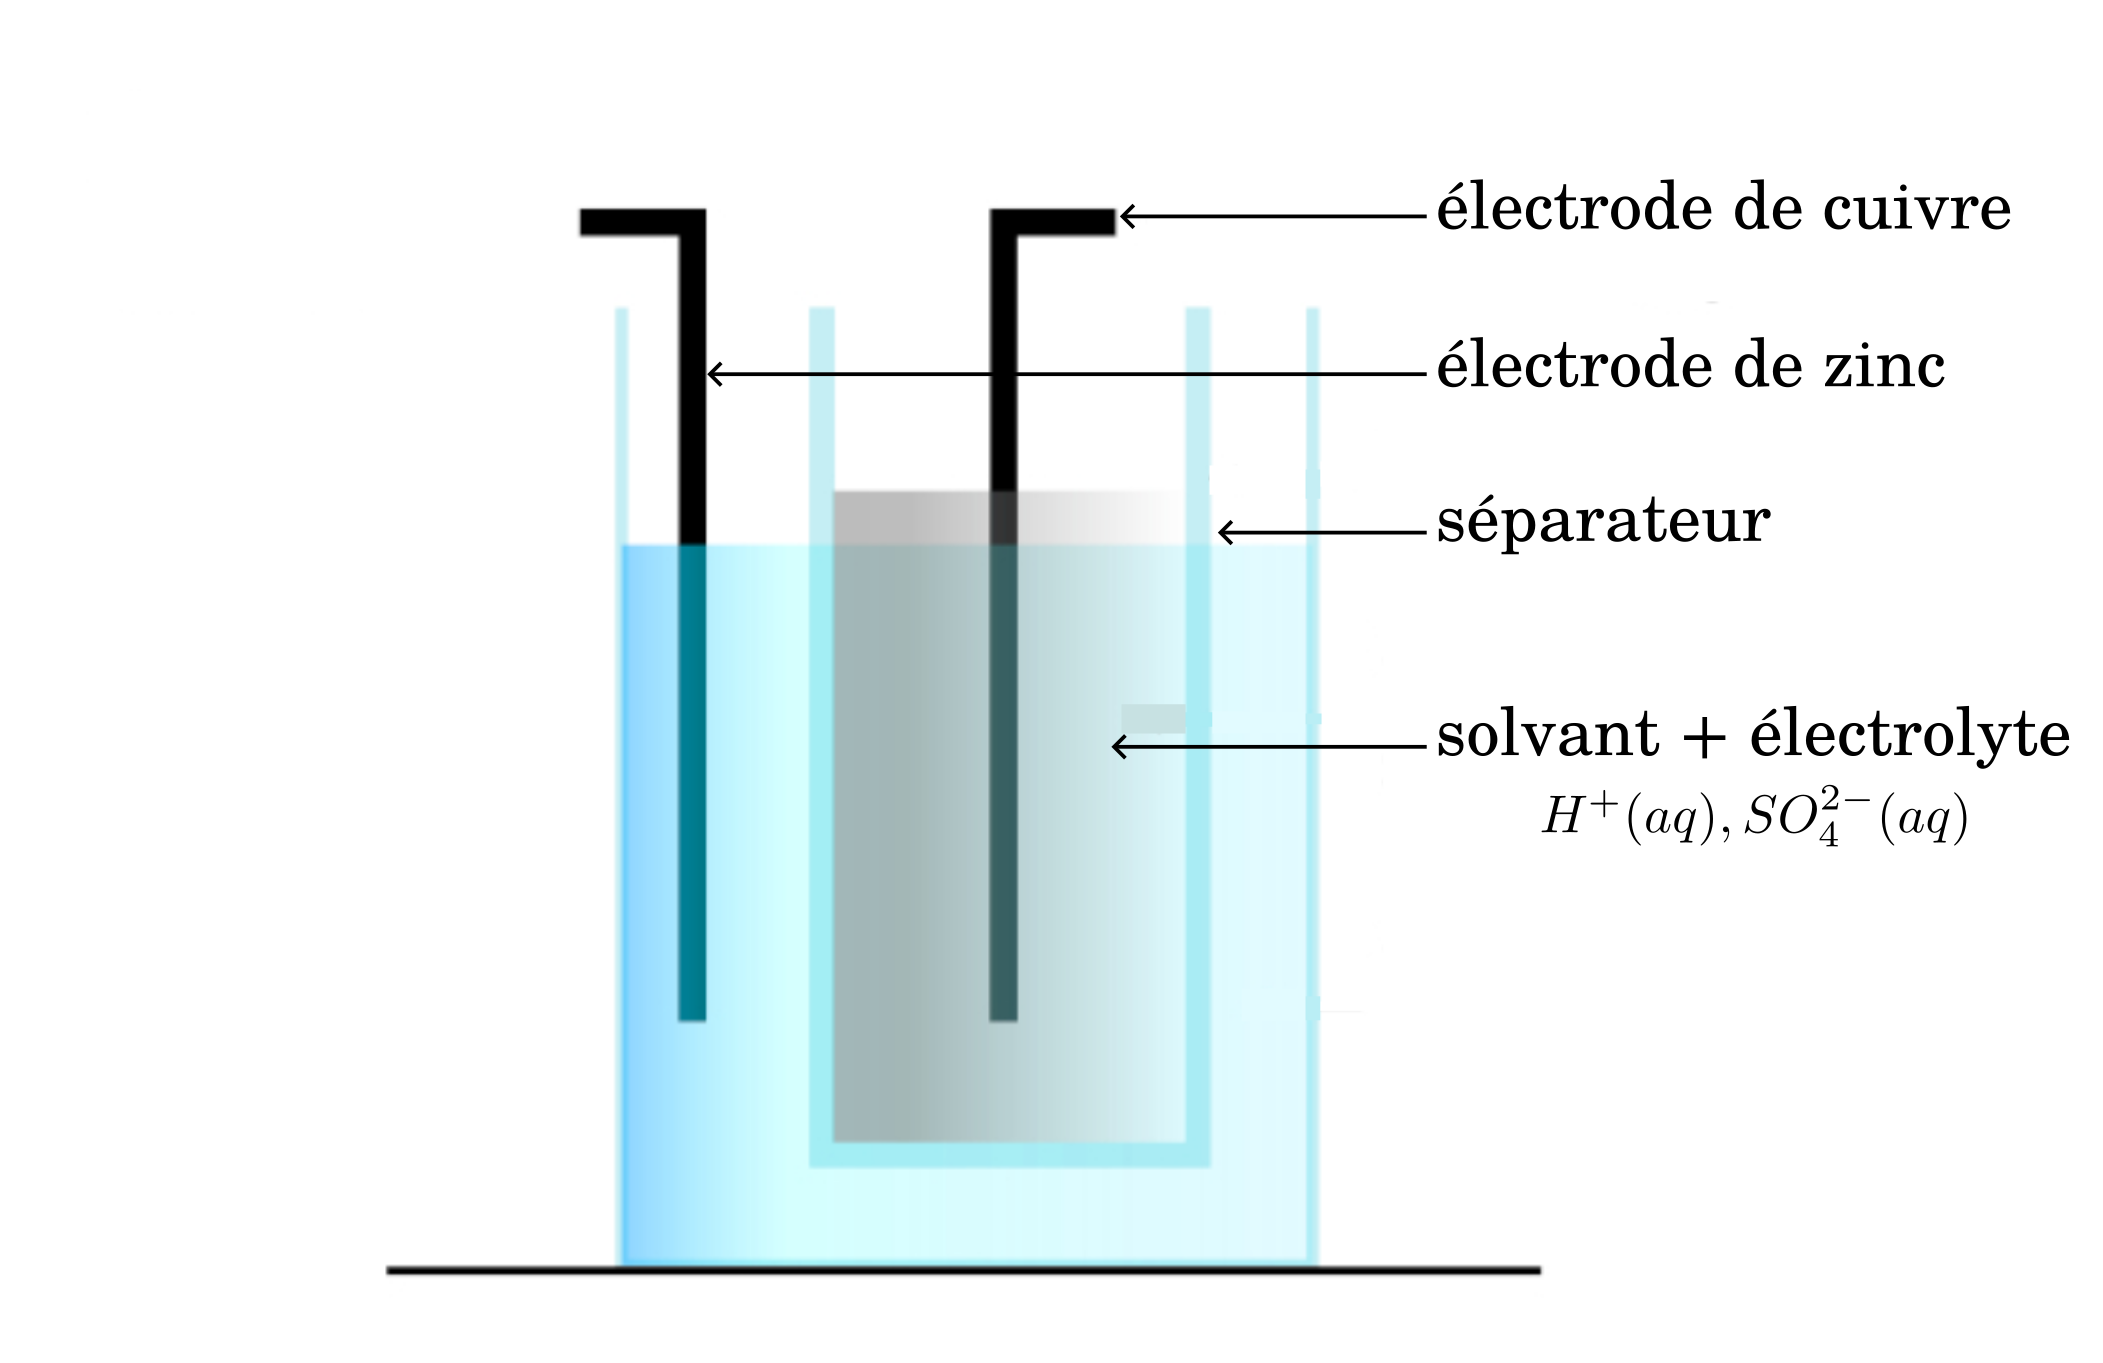
\includegraphics[width=\textwidth]{Ex35/Fig01-Correction}
\end{minipage}\hfill\begin{minipage}{0.48\textwidth}
\captionof{figure}{Schéma d'une pile Daniell legendée}
\end{minipage}
\end{center}
Chacune demi-pile doit être explicitement associée au compartiment anodique et au compartiment cathodique. Le collecteur de courant n'apparaît pas explicitement dans ce schéma, mais il s'agira des pièces assurant la jonction entre le circuit électrique et une des électrodes.
}

\cteacher{Vous pouvez éventuellement vous commenter l'orientation de la pile en vous appuyant sur la noblesse de chacun des métaux. Puisque le zinc est beaucoup moins noble que le cuivre, cette électrode jouera le rôle d'anode (oxydation), tandis que le cuivre jouera le rôle de cathode.}



\Q La pile saline est une cellule contenant un électrolyte gélifié de chlorure de zinc \ce{ZnCl2} et de chlorure d'ammonium \ce{NH4Cl}. Les électrodes sont en zinc et en oxyde de manganèse.

\begin{center}
\begin{minipage}{0.48\textwidth}
\centering

\includegraphics[width=0.8\textwidth]{Ex35/Fig03}
\end{minipage}\hfill\begin{minipage}{0.48\textwidth}
\captionof{figure}{Schéma d'une pile saline}
\end{minipage}
\end{center}

\solution{On peut proposer la légende suivante : 
\begin{center}
\begin{minipage}{0.48\textwidth}
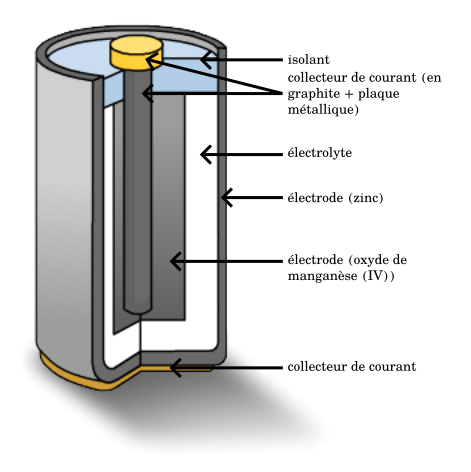
\includegraphics[width=\textwidth]{Ex35/Fig03-Correction}
\end{minipage}\hfill\begin{minipage}{0.48\textwidth}
\captionof{figure}{Schéma d'une pile saline legendée}
\end{minipage}
\end{center}
Chacune demi-pile doit être explicitement associée au compartiment anodique et au compartiment cathodique. Ici l'électrolyte étant solide (gel), il y a bien séparation entre l'oxyde et le zinc. De plus, le collecteur de courant en graphite ne descent pas jusqu'au pôle $\ominus$. Il semble que lorsque c'est le cas, un séparateur soit ajouté.
}

\Q L'accumulateur li-ion est une cellule contenant un électrolyte de sels de lithium en milieu organique. Les électrodes sont en graphite ithié et en oxyde métallique lithié.

\begin{center}
\begin{minipage}{0.48\textwidth}

\includegraphics[width=0.8\textwidth]{Ex35/Fig02.png}
\end{minipage}\hfill\begin{minipage}{0.48\textwidth}
\captionof{figure}{Schéma d'un accumulateur li-ion}
\end{minipage}
\end{center}

\solution{On peut proposer la légende suivante : 
\begin{center}
\begin{minipage}{0.48\textwidth}
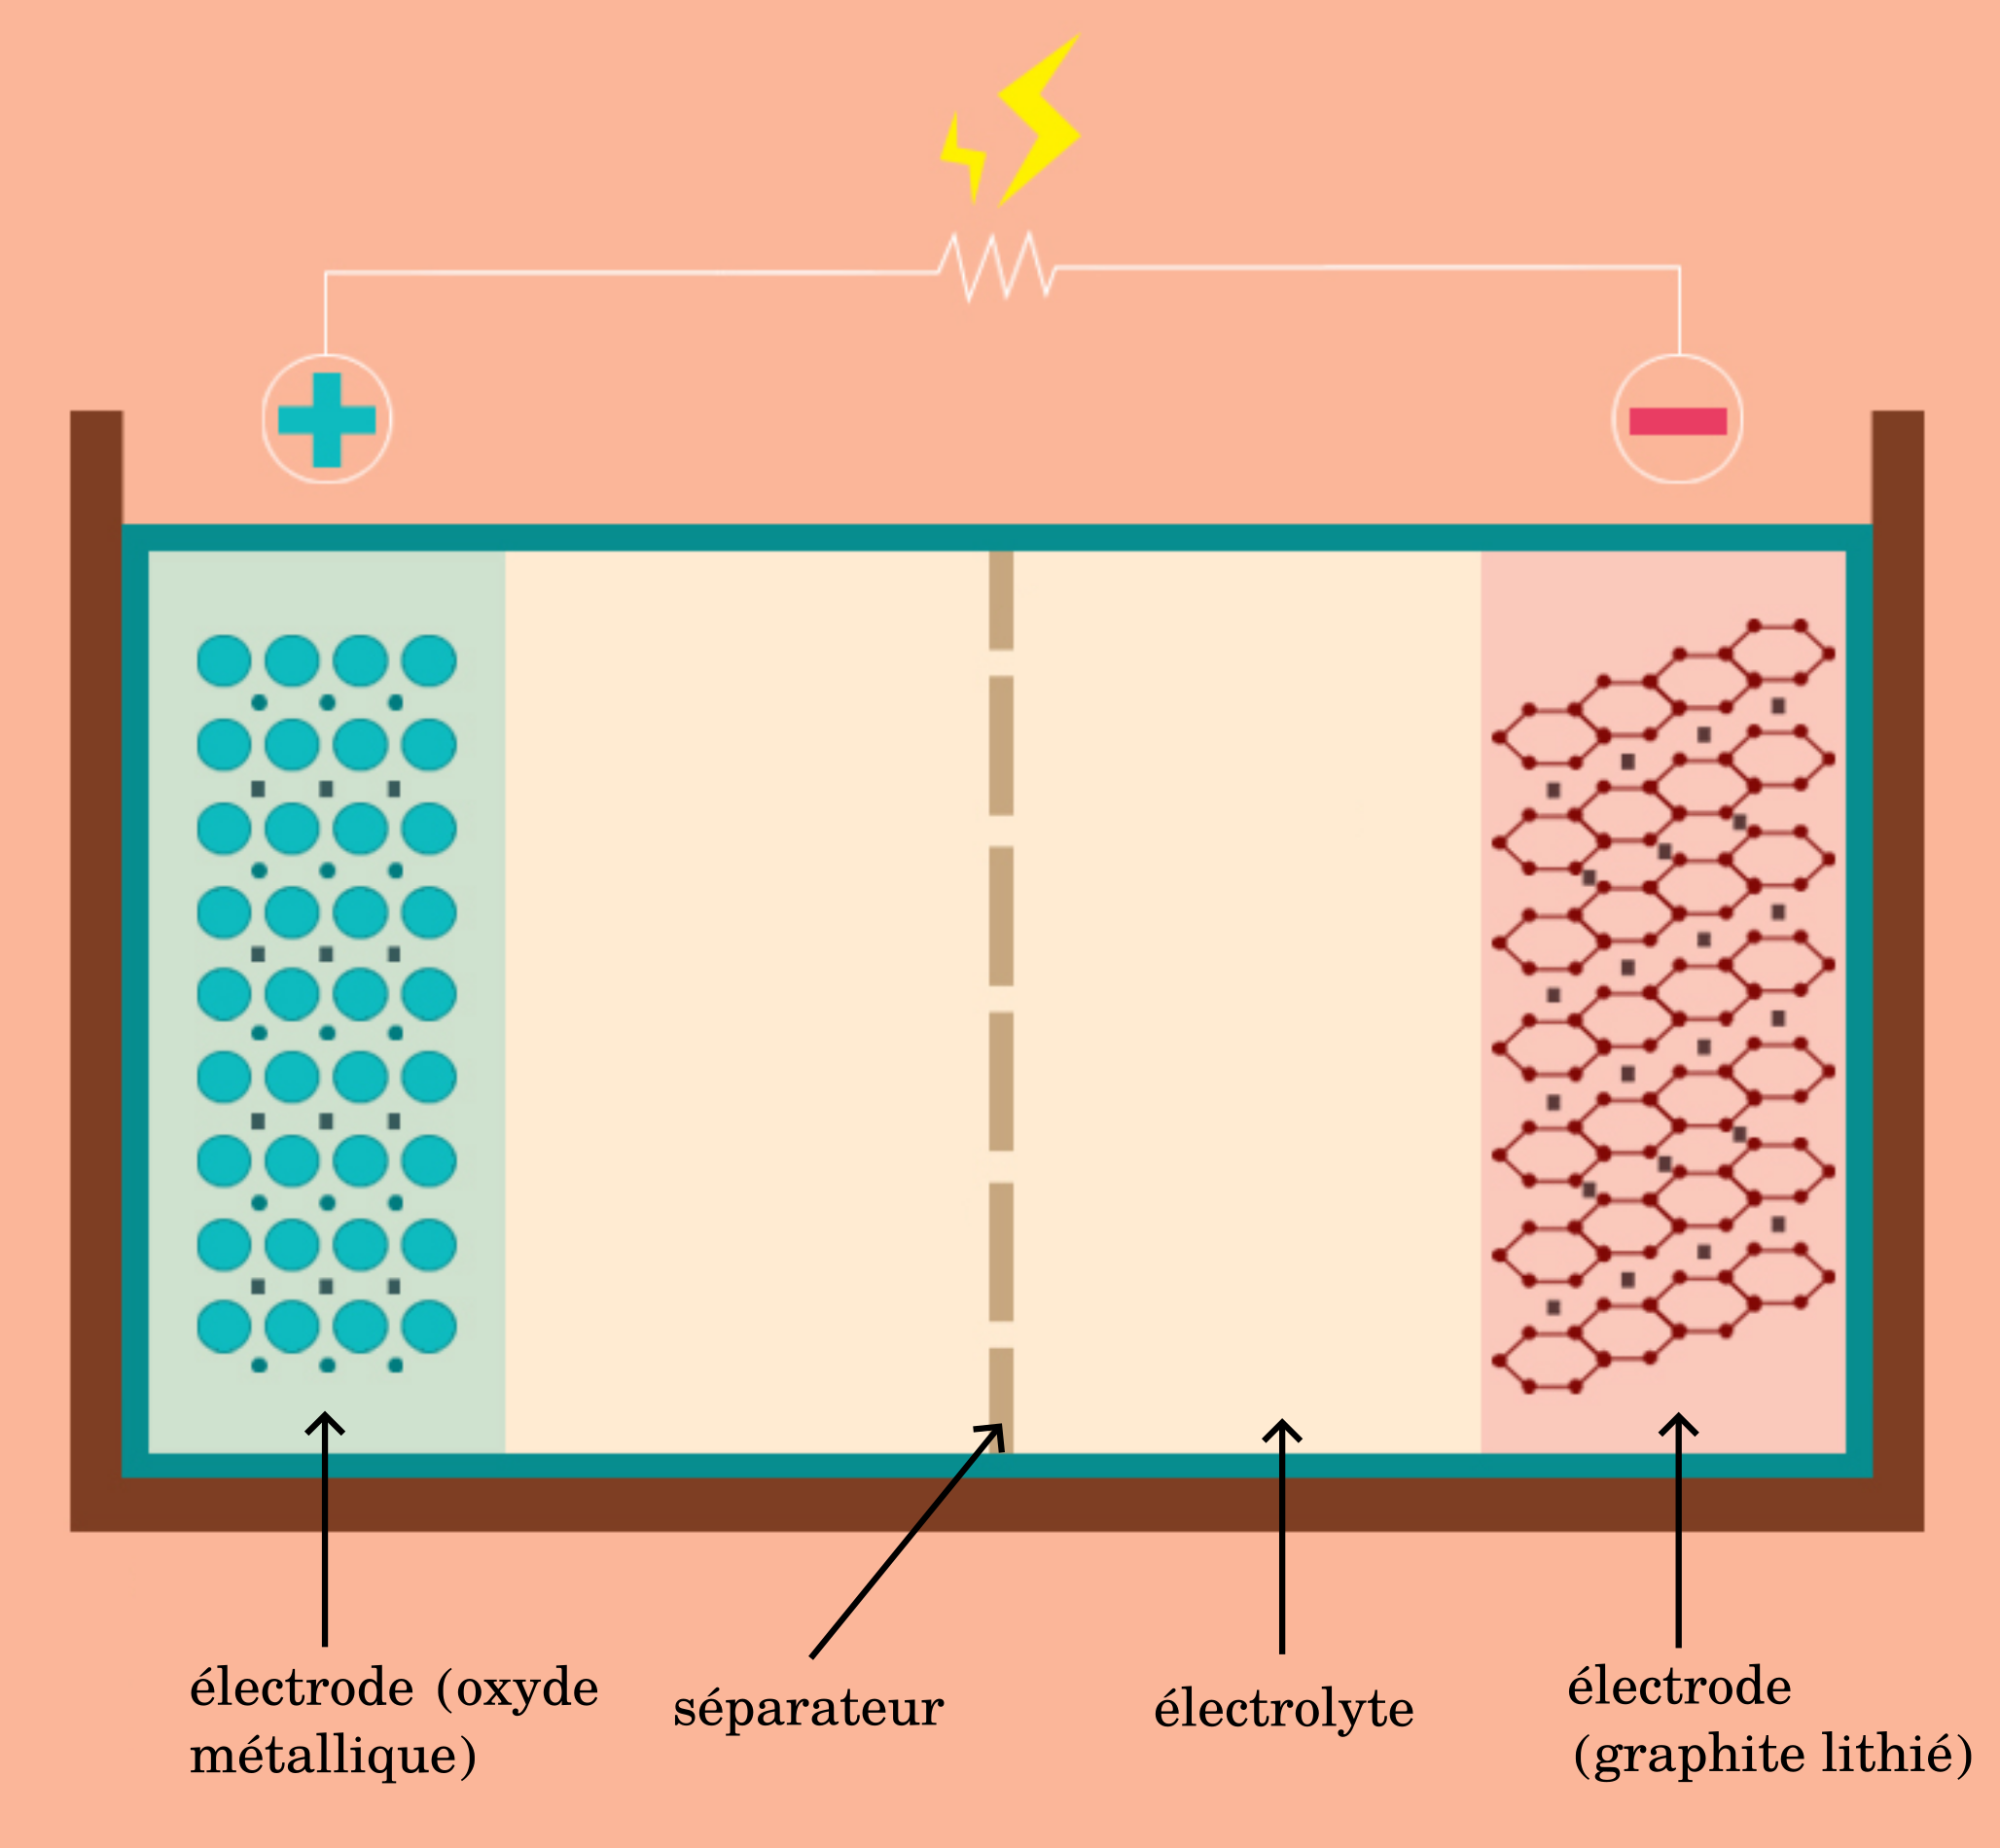
\includegraphics[width=\textwidth]{Ex35/Fig02-Correction}
\end{minipage}\hfill\begin{minipage}{0.48\textwidth}
\captionof{figure}{Schéma d'un accumulateur au lithium}
\end{minipage}
\end{center}
Les collecteurs de courant n'apparaissent pas explicitement dans ce schéma, bien qu'il y en ait forcément à chaque pôle.
}

\cteacher{Attention, vous pouvez insister sur le fait que les électrodes peuvent résulter de formulations plus complexe qu'un unique matériau. Par exemple, dans la pile saline, on mélange souvent l'oxyde de manganèse avec du graphite pour améliorer les propriétés de conduction électrique.
En TP, ils seront emmenés à faire de même avec leur cathode.
}
